\begin{figure}[H]
\centering
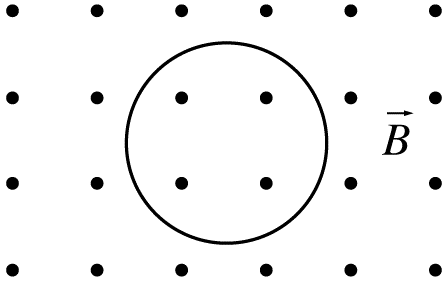
\includegraphics[scale=0.3]{images/img-010-031.png}
\end{figure}

% Multiple Choice Question 19
\begin{questions}\setcounter{question}{18}\question
A uniform magnetic field $\vec{B}$ is directed out of the page, as represented above. A loop of wire of area $0.8 \unit{m^2}$ is in the plane of the page. At a certain instant, the field has a magnitude of $5.0 \unit{T}$ and is decreasing at the rate of $0.5 \unit{T/s}$. The magnitude of the induced emf in the wire loop at this instant is most nearly

\begin{oneparchoices}
\choice $0.4 \unit{V}$
\choice $1.6 \unit{V}$
\choice $2.0 \unit{V}$
\choice $4.0 \unit{V}$
\choice $8.0 \unit{V}$
\end{oneparchoices}\end{questions}

